\section{Architecture instantiated}\label{sec:proposed-architectures}
For the development of this proposal, two neural network architectures have been proposed by instantiating the architectural model defined in the previous section: instance with One-Class classification (D-ADV-OC) and instance with Multi-Class classification (D-ADV-MC). These architectures are able to detect specific behaviors that are part of the training data set and abnormal behaviors from training normal data, respectively. Details about the classification and training stages, as well as some important configuration parameters of each of the architecture instances, are explained in the subsections \ref{subsec:arq-mcc} and \ref{subsec:arq-occ}.

\subsection{Multi-activity classification (D-ADV-MC)}\label{subsec:arq-mcc}

\begin{figure*}[htbp]
	\centerline{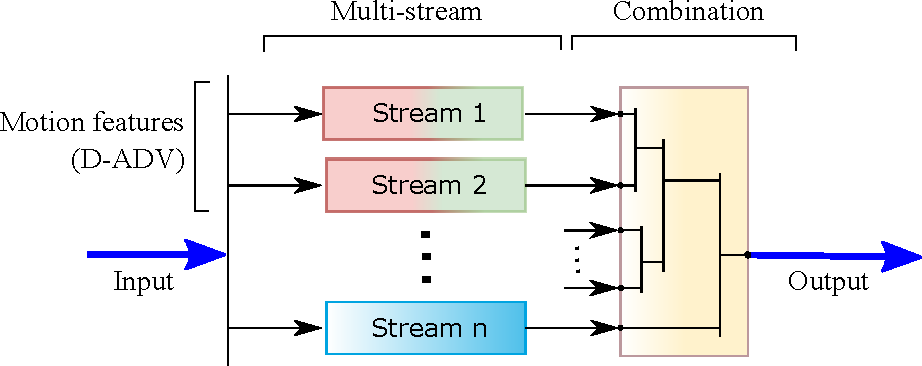
\includegraphics[width=0.9\textwidth]{images/placeholder_figure.pdf}}
	\caption[Data flow in the D-ADV-MC]{Data flow of the proposed D-ADV. The D-ADV architecture is mainly divided into two parts, the D-ADV-MC representation stage where the displacement is calculated using the ADV descriptor from a sequence of images and their optical flow motion. The second stage defines the classifier using CNN classifiers and a fully connected layer to predict the class.}
	\label{fig:pipeline}
\end{figure*}
The architecture instantiated from the architectural model proposed in this paper for the classification of multiple group activities can be seen in Figure \ref{fig:pipeline}. This architecture uses two-stream activity classification and performs a late fusion as discussed in the previous section capable of classifying the previously computed D-ADV images: $LRF$ and $UDF$. The classifier approach is open and allows the use of any CNN architecture (VGG, Resnet, Alexnet, LeNet, etc.). This type of networks typically uses a fully connected layer on the output with a softmax activation function to decide to which class the image corresponds (e.g. objects, locations, poses, etc.). The architecture ignores the individual dense layers. However, the previous layers of the model are concatenated in a late merge with a fusion layer. Finally, we use a fully connected layer with sigmoid activation function to connect the fusion layer and predict multiple classes.

To overcome the challenge of training the architecture with small datasets such as BEHAVE and CAVIAR \cite{fisher2004pets04, blunsden2010behave}, we perform transfer learning of the trained models with the ImageNet dataset \cite{krizhevsky2012imagenet}. As a result, we refined the CNN-based network three times. First, we replaced the fully connected layer of the ImageNet architecture with a new one that matches our classes. Second, we trained a subset of the lower layers because the $LRF$ and $UDF$ inputs are different from the $RGB$ input images expected by ImageNet. Finally, we retrained a subset of the upper layers for fine-tuning.   

For the training step, we use the binary cross-entropy as an objective function to consider each output class as an independent Bernoulli distribution. For classification, considering that more than one class can be present in a time frame of the sequence, different thresholds $\epsilon_i$ are considered for each output neuron $i$. Here the $\epsilon_i$ thresholds are calculated to be the value that maximises the true positive rate ($TPR$) and minimises the false positive rate ($FPR$), for each class, $C_i$.

\subsection{Abnormal Activity Classification (D-ADV-OC)}\label{subsec:arq-occ}

\begin{figure*}[htbp]
	\centerline{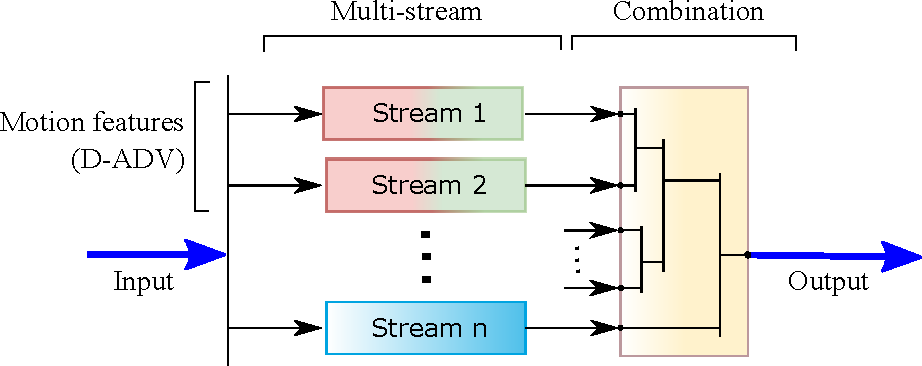
\includegraphics[width=0.9\textwidth]{images/placeholder_figure.pdf}}
	\caption[Data flow in the D-ADV for D-ADV-OC]{The data flow of the D-ADV-OC method. The D-ADV-OC architecture is mainly divided into two parts, the D-ADV-OC representation stage where the displacement is calculated using the ADV descriptor from a sequence of data and its optical flow movement. The second stage defines the classifier using CNN classifiers and a fully connected layer to identify the class whether it is normal or abnormal.}
	\label{fig:pipeline-occ}
\end{figure*}

This section specifies the instance of the proposed architecture for the detection of anomalous activities in a scene. This architecture uses three data streams: the two motion-related streams from the D-ADV with the $LRF$ and $UDF$ images, and the a third stream associated with the scene context. This architecture has been coined D-ADV-OC, and does not use the individual dense layers as it connects to layers upstream of them. Therefore, the upstream layers in the convnet are concatenated in a late merging manner using a concatenation layer of the two streams. After all, we use a fully connected layer with linear activation to connect the concatenation layer and predict abnormal activity in the cluster. This architecture design is based on recent work by Ruff et al. \cite{pmlr-v80-ruff18a} providing a deep model for training a neural network by minimizing the volume of a hypersphere enclosing the data network representations. This proposal differs from the work of Chalapathy et al. \cite{chalapathy2018anomaly} by combining the ability of CNN-based networks to progressively learn from a subset of images that are the representation of the input data along with the one-class target. Unlike the latter work, which uses auto-encoders to establish the representation of the input data by defining the center of the hypersphere, in this paper some layers of the CNN-based network are trainable, allowing the architecture to continue training both the center and adjusting the radius of the hypersphere. To avoid the problems of large datasets to train our model and with the goal that it can be used for small datasets, transfer learning of the models trained with ImageNet is used.

The third stream of this architecture is related to the context information in the scene, and at the training step, we calculate the maximum values of the input patterns to normalize the output data, which could be objects, locations, etc. The mean value of the normalization establishes the center of the hypersphere, optimizing the length of the hypersphere radius by means of a fully connected layer at the end of the network.

The distance combination module (see Figure \ref{fig:pipeline-occ}) uses the weights $w_a$ and $w_c$ for the activity and context loss functions to train the network and calculates the distance of an input pattern to the normal class according to the prediction stage using the following function:
$$ dist = \frac{1}{n} w_a \sum_{i}{||i_a - c_a ||^2 + w_c|||i_c - c_c |^2 }$$ 
where $i_a$ is the computed representation for the activities using motion; $i_c$, the computed representation of the context in the scene; and, finally, $c_a$ and $c_c$ are the centers of the hyperspheres. Additionally, in this model, the combination of the weights $w_a$ for behavior and $w_b$ are taken into account.
